\section{Genomförande} % (fold)
\label{sec:genomf_rande}
    \subsection{Fas 1} % (fold)
    \label{sub:steg_1}
        Projektet genomfördes med stöd av den valda metoden. I problemidentifikations-fasen, fas ett, hölls möten med uppdragsgivaren i syfte att få en enhällig uppfattning om vad företaget efterfrågade och formaliserade det praktiska problem som företaget sökte en lösning till. Vidare är det även i den här fasen som introduktionen till projektets rapport utvecklades för att fastslå vad projektet avser att utföra, som ett led i problemidentifieringen. \bigskip

        Den initiala problemanalysen resulterade i att projektet i stort kommer vara uppdelat i två mindre delar, dels den algoritm som klarar av att kalibrera panelen och dels en kommunikationslösning mellan panelen och rummet som den levererar ljuset till. \bigskip

        Förutsättningen vid litteraturstudien, gällande kommunikationen mellan taket och byggnadens innandöme, var att den trådlösa kommunikationen skall ske med standardiserade protokoll. Detta för att underlätta mottagandet av den trådlösa sändningen, i syfte att undvika tidssänken i felsökning då projektet har en relativt snäv tidsram.\bigskip

        För kalibreringsalgoritmens del bestod problemförståelsesteget av att undersöka vilka typer av datastrukturer som skulle komma att beröras. När problemet analyserades insågs att värdena som samlas in kan representeras som en tvådimensionell matris (eng. 'array'), där det finns ett unikt maxvärde och kring detta minskande värden som blir lägre ju längre från maxvärdet de befinner sig, se figur\ref{fig:array}. \bigskip

        \begin{figure}[hbt]
        \centering
            \begin{subfigure}{0.2\textwidth}
                \pgfplotstabletypeset[color cells={min=5,max=9}, /pgfplots/colormap={yellowred}{rgb255(0cm)=(255,255,105); rgb255(1cm)=(255,10,10)},]
                {
                    5   6   7   6
                    6   7   8   7
                    7   8   9   8
                    6   7   8   7
                }
            \end{subfigure}
            \begin{subfigure}{0.2\textwidth}
                \pgfplotstabletypeset[color cells={min=3,max=9}, /pgfplots/colormap={yellowred}{rgb255(0cm)=(255,255,105); rgb255(1cm)=(255,10,10)},]
                {
                    6   7   8   9
                    5   6   7   8
                    4   5   6   7
                    3   4   5   6
                }
            \end{subfigure}
        \caption{\label{fig:array} Exempel på förväntade matriser}
        \end{figure}
    % subsection steg_1 (end)


    \subsection{Fas 2} % (fold)
    \label{sub:steg_2}
        Litteraturstudien resulterade i en förståelse att trådlösa standarder för datakommunikation så som 802.11 standarderna har problem att sända när betongkonstruktioner hindrar utspridningen av radiovågorna och kräver speciell apparatur för att klara av att skicka data igenom sådana förhållanden \cite{11n}. Detta medför att trådlös kommunikation inte är lämplig för företaget, då de på förhand inte kan veta ifall deras kommunikation kommer att fungera på plats hos deras kunder. Inköp av nämnda apparatur är inte aktuellt. \bigskip

        Ett lämpligare medium att kommunicera via är istället de fiberoptiska kablar som redan är dragna, då rummet lyses upp av just dessa kablar. Enligt företaget kommer det finnas mer än en fiberkabel dragen till varje rum, vilket öppnar upp för möjligheten att koppla in apparatur för kommunikation i en fiberkabel, medan den eller de andra kablarna kan fortsätta hämta in ljus till rummet. Med de svårigheter som den trådlösa kommunikationen medförde i kombination med att ett fungerande alternativt medium redan finns draget, valde projektet att fokusera på det senare. När ''val av tillämpningar'' genomfördes för kommunikationen, konstaterades det att panelens fiberändar har ett reflekterande skydd mot infrarött ljus, enligt \ref{ssub:fiberoptik}, och att ultraviolett ljus inte leds genom panelens yttre glasskiva, vilket leder till att kommunikationen över fiberkabeln måste ske med ljus i det synliga spektrumet. \bigskip

        Gällande kalibreringsalgoritmen framstod det vid datorkörningar att en algoritm som itererar över hela matrisen för att leta det högsta värdet kommer att vara väldigt ineffektiv. Ett beslut fattades om att utveckla en algoritm som kräver så få steg som möjligt, detta då den praktiska implementationen kommer att innebära fördröjningssteg vid två punkter i körningen, dels när panelen flyttar på sig, och dels när ljuset ska hämtas in från luxmätaren. Algoritmen ska kontinuerligt söka efter ett högre värde tills det maximala värdet är funnet, likt figur~\ref{fig:array}.
    % subsection steg_2 (end)


    \subsection{Fas 3} % (fold)
    \label{sub:steg_3}
        Genom att fokusera på det optiska alternativet vid kommunikation mellan panelen och rummet, ledde detta in projektet till det tredje steget i metoden, att föreslå en artefakt som löser det ställda problemet. 

        \subsubsection{Utformning av kommunikationslösning} % (fold)
        \label{ssub:utformning_av_kommunikationslosning}
            Kommunikationsdelen i projektet har genomgått flera iterationer av fas 3 och två huvudlösningar presenterades.\bigskip 

            Den första lösningen som projektet föreslog är en en lösning med en mikrokontroller inne i det upplysa rummet som omvandlar från en luxmätares utdata till en optisk signal, som sänds upp till panelen  för att där avkodas. När signalerna skickas via fibrerna kommer ljuset att stråla ut ur solpanelens linser, vilket då en mottagare kan analysera. Monterad på panelen är mottagaren även den en mikrokontroller, med en ljuskänslig sensor som omvandlar de optiska signaler från sändaren, till digitala signaler. Mottagaren skickar då vidare den digitala datan till den enhet som utför den algoritm som avser kalibrera solsensorn. \bigskip

            Den andra lösningen är att istället för att mäta upp ljusstyrkan i rummet, koppla ihop två stycken optiska fibrer från samma panel i rummet, vilket då skickar upp ljusintaget tillbaka till panelen. Genom att täcka över de linser som förser den ena fiberkabeln med ljus, kommer den andra fiberkabeln att skicka ut dess ljusintag, via de nu täckta linserna. I detta förslag kan en luxmätare sitta i övertäckningsanordningen och där mäta upp hur mycket ljus panelen tar emot, via omvägen till det upplysta rummet och tillbaka. Då luxmätaren nu befinner sig på panelen, kan den direkt skicka sin data till den enhet som förväntas utföra algoritmen. %\bigskip
        % subsubsection utformning_av_kommunikationslosning (end)

        \subsubsection{Programmeringsspråk} % (fold)
        \label{ssub:programmeringssprak}
            Programmeringsspråket som valdes för utveckling av algoritmen var \texttt{Python} och valet hade stöd av flera motiveringar. Den första anledningen till att språket valdes var att företaget har kompetens och erfarenhet att utveckla i detta språk, då den nya panelen SP4 kommer att drivas av en källkod skriven i just \texttt{Python}. Att kompetens och kunskap finns inom företaget medför att applikationen kan underhållas av företaget själv och modifieras vid framtida behov. Vidare har företaget sedan tidigare produkter utvecklade i detta programmeringsspråk, så att utveckla algoritmen i samma språk underlättar för en eventuell implementering av algoritmen i de existerande produkterna. Mer generella fördelar med att utveckla i \texttt{Python} är att språket är plattformsoberoende och är enkelt att utveckla grafiska gränssnitt i. Nackdelar med språket är att det är långsamt i förhållande till andra språk så som \texttt{C} eller \texttt{Java} men då algoritmen kommer att kommunicera med mekanik, vilket leder till flertalet inbyggda fördröjningar för rotation av panelen och inhämtning och sändning av information, ser projektet att språkets åverkan på hur snabbt algoritmen kan utföras som försumbar \cite{python_speed}. %\bigskip
        % subsubsection programmeringssprak (end)

        \subsubsection{Utveckling av algoritm} % (fold)
        \label{ssub:utveckling_av_algoritm}
            Utformningen av algoritmen skedde genom flera iterationer av steg 3 i den valda metoden. I den första iterationen utvecklades en sökalgoritm, algoritm $\mathscr{A}$, som inledningsvis genomsöker en 3x3-matris i syfte att finna en inledande sökriktning. Därefter genomförs sökning medurs i åtta riktningar med utgångsriktning motsvarande österut. När ett större värde påträffas uppdateras nuvarande position och sökningen återupprepas. För jämförelse utvecklades även en variant med fyra sökriktningar, algoritm $\mathscr{B}$. Efterkommande iterationer var samtliga en vidareutveckling av den förra. Den andra iteration vidareutvecklade algoritmen så att den lagrar information om tidigare besökta koordinater, så att dessa ej undersöks vid upprepade tillfällen. Ytterligare förbättringar implementerades i den tredje iterationen, då riktningen på den senaste förflyttningen, då ett nytt större värde påträffats, registreras. Med hjälp av denna information undersöks först samma riktning som den senast lyckade förflyttningen innan medurs sökning. Här slopades också den inledande sökningen i 3x3 matris, då den inte kunde påvisas ha några märkbara fördelar. Samtliga iterationer innebar märkbara förbättringar vid simulering. Den slutgiltiga algoritmen arbetar enligt det flödesschema som finns presenterad i bilaga~\ref{sec:sokalgoritm_flow}. %\bigskip
        % subsubsection utveckling_av_algoritm (end)

        

        \subsubsection{Utvärdering av algoritm} % (fold)
        \label{ssub:utvardering_av_algoritm}
            \begin{figure}[ht!]
                \pgfplotsset{width=8cm,compat=1.8}
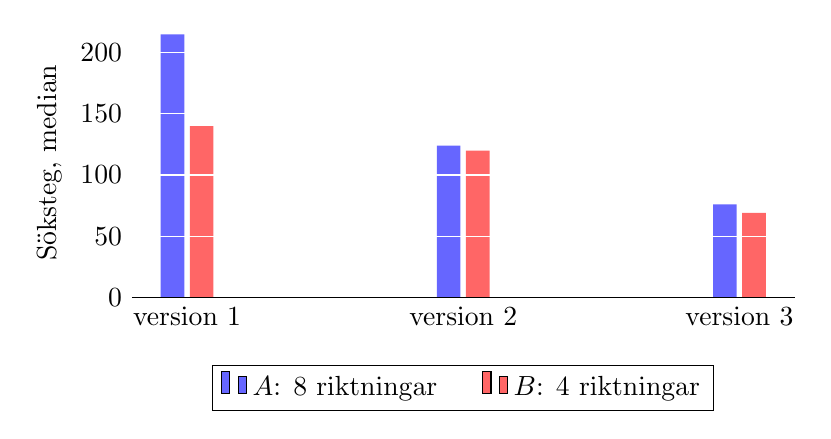
\begin{tikzpicture}
    \centering
    \begin{axis}[
        ybar,
        axis on top,
        % title={Söksteg algoritmer},
        height=5cm, width=10cm,
        bar width=0.3cm,
        ymajorgrids, tick align=inside,
        major grid style={draw=white},
        enlarge y limits={value=.1,upper},
        ymin=0, ymax=200,
        axis x line*=bottom,
        axis y line*=left,
        y axis line style={opacity=0},
        tickwidth=0pt,
        enlarge x limits=true,
        legend style={
            at={(0.5,-0.25)},
            % font=\footnotesize,
            anchor=north,
            legend columns=2,
            /tikz/every even column/.append style={column sep=0.5cm}
        },
        ylabel={Söksteg, median},
        symbolic x coords={version 1, version 2, version 3},
        xtick=data,
        % tick label style={font=\footnotesize},
        ]
        
        %% Median 8 riktningar
        \addplot [draw=none,fill=blue!60] coordinates {
            (version 1,215)
            (version 2,124) 
            (version 3,76)
        };

        %% Median 4 riktningar
        \addplot [draw=none, fill=red!60] coordinates {
            (version 1,140)
            (version 2,120) 
            (version 3,69)
        };
        \legend{$\mathscr{A}$: 8 riktningar,$\mathscr{B}$: 4 riktningar}
    \end{axis}
\end{tikzpicture}
            \caption{\label{fig:algoritm_steg} Jämförelse algoritmernas antal söksteg}
            \end{figure}

            För att jämföra sökalgoritmer genomfördes simuleringar för att mäta det antal steg som behövs för att ta sig från utgångspositionen till den position där det maximala värdet påträffades. Simuleringarna använde sig av 10\thinspace000 100x100-matriser där varje matris hade en slumpvis genererad utgångsposition och maximalt värde. Algoritmerna har alltså alla genomsökt samma matriser med samma utgångspositioner. Samtliga positioners värden var strängt avtagande i hänseende till avståndet från det maximala värdet. För varje iteration av algoritmen undersöktes sökning med både fyra och åtta sökriktningar. Sökning i fyra riktningar visade sig mer effektivt i samtliga fall, enligt figur~\ref{fig:algoritm_steg} och bilaga~\ref{sec:sokalgoritm_sim}. Skillnaderna i antal steg mellan samma algoritm med olika antal sökriktningar vara störst i den första iterationen, med 54~\% fler steg, men de visade sig även i övriga iterationer. I den tredje och slutgiltiga iterationen var skillnaden 10~\% fler steg. Varje iteration av algoritmen minskade det antal steg som behövdes för att finna det största värdet. Största förändringen mellan iterationer skedde mellan iteration två och tre, där antalet steg minskades med 43~\%, se tabell~\ref{tab:algoritm_forbattring}. Minskningen mellan iteration ett och tre var 51~\%. \bigskip

            \begin{table}[b]
                \caption{\label{tab:algoritm_forbattring}Minskning av antal steg mellan varje version}
                \centering
                \begin{threeparttable}
                \begin{tabular}{@{}lcc@{}}
                \toprule
                Från        & \multicolumn{1}{l}{Till version 2} & \multicolumn{1}{l}{Till version 3} \\ \midrule
                Version 1 & 14~\%                                & 51~\%                                \\
                Version 2 & -                                    & 43~\% \\ \bottomrule
                \end{tabular}
                \begin{tablenotes}
                \item Baserat på medianvärden, se bilaga~\ref{sec:sokalgoritm_sim}
            \end{tablenotes}
            \end{threeparttable}
            \end{table}

            För att testa algoritmen på solpanelen genomfördes först en simpel genomsökning av panelens solintag till en tvådimensionell matris, i syfte att undersöka ifall utformningen av panelens fokuspunkt överensstämmer med projektets antagande i figur~\ref{fig:array}. Resultatet av denna sökning gav en annorlunda bild av hur fokuspunkten ser ut från panelen, vilket visas i figur~\ref{fig:array1}. För fullständig data av denna sökning, se bilaga~\ref{sec:heatmap}. Trots att fokuspunkten inte är utformad på samma sätt som förutspått, fungerar sökalgoritmen så pass att den riktar in sig till det högsta funna värdet, dock på grund av panelens utformning av fokuspunkten finns det inget exakt högsta värde, utan algoritmen stannar i en punkt i den cirkel som panelen genererar. Algoritmen är inte utformad för att söka igenom hela cirkeln och sätta det högsta värdet, utan lokaliserar ett lokalt maximum. Detta ger ett högt belysningsvärde ut från panelen även om det kan finnas ett något högre värde existerar på motsatt sida av cirkeln. Skillnaden inom denna cirkel är dock så pass små att det rör sig om så små värdeskillnader att dessa kan anses ligga inom felmarginalen. Att utveckla en algoritm som arbetar sig igenom hela cirkeln är fullt möjlig, men det handlar om en avvägning om hur lång tid kalibreringen kommer ta, den nu gällande algoritmen är utvecklad för att hitta ett lokalt maximum på så få steg som möjligt.
        

            \begin{figure}
            \centering
                \setlength{\fboxsep}{0pt}
                \fbox{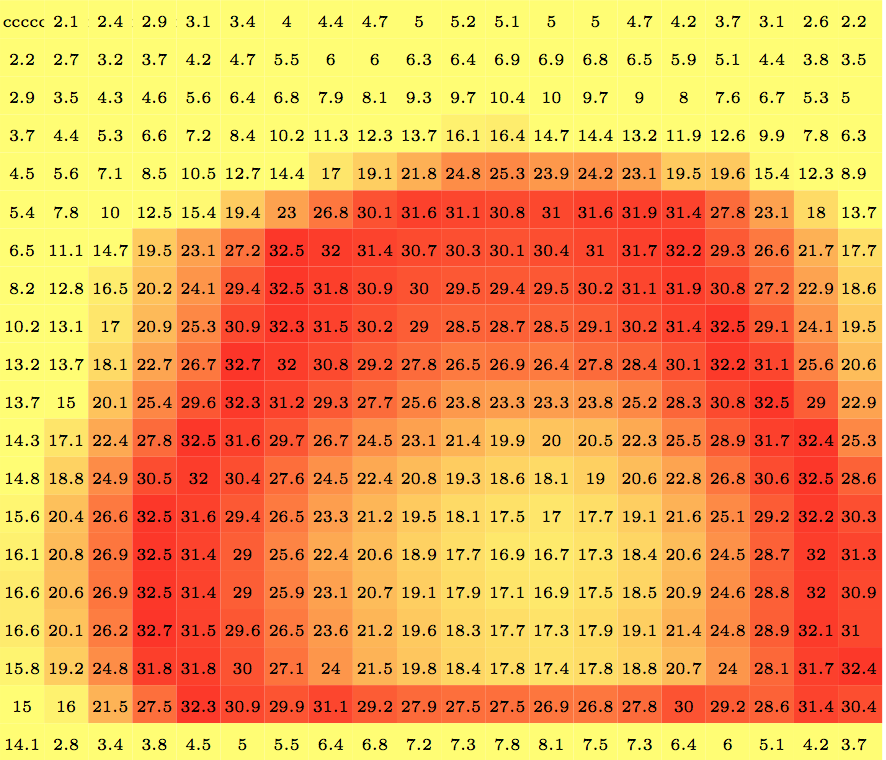
\includegraphics[scale=0.25]{res/img/heatmap1}}
                \caption{\label{fig:array1}Översikt av uppmätt fokuspunkt}
            \end{figure}
        % subsubsection utvardering_av_algoritm (end)

        \subsubsection{Utveckling av kommunikationslösning} % (fold)
        \label{ssub:utveckling_av_kommunikationslosning}
        % subsubsection utveckling_av_kommunikationslosning (end)

        \subsubsection{Avläsning av luxmätare} % (fold)
        \label{ssub:avlasning_av_luxmatare}
        % subsubsection avlasning_av_luxmatare (end)

        \subsubsection{Utveckling av applikation} % (fold)
        \label{ssub:utveckling_av_applikation}
            Efter att ha implementerat en algoritm som i simuleringar uppfyllde önskvärd funktion påbörjades utveckling av en applikation där den kan tillämpas. Förutom själva kalibreringsalgoritmen skulle applikationen ha egenskaper som kommunikation med panelen, ett användarvänligt grafiskt gränssnitt och inhämtning av värden från luxmätare. Applikationen utvecklades i version 3.4 av programmeringsspråket \texttt{Python} av anledningar nämnda i \ref{ssub:programmeringssprak}. \bigskip

            För att kommunicera med panelen och den Arduino som mottar värden från luxmätaren Adafruit TSL2591 behövdes stöd för seriell kommunikation. Ett bibliotek som möjliggjorde seriell kommunikation med enheter anslutna till en dator var pySerial. Eftersom pySerial har stöd för operativsystem baserade på Windows, Linux och BSD är biblioteket i praktiken plattformsoberoende \cite{pyserial}. \bigskip

            Ett beslut behövdes tas om ramverk för grafiskt gränssnitt. Till ändamålet fanns flera ramverk utvecklade och anpassade till \texttt{Python}. Det som ansågs mest lämpligt för applikation var TkInter, där en anledning är att Parans sedan tidigare har kringutrustning som använder TkInter \cite{solarremote}. Hänsyn togs till att underlätta både framtida hantering av koden för bolaget och en eventuell integrering av tidigare produkter med den av projektet utvecklade applikationen. En annan anledning är att ramverket distribueras med standardinstallationer av \texttt{Python} till Windows och Mac OS X \cite{tkinter}. Till Linuxsystem installeras TkInter separat och det finns tillgängligt i flera stora Linuxdistributioners pakethanterare. Behovet av extra installationer för ett ramverk kunde minimeras och det grafiska gränssnittet kunde göras plattformsoberoende. \bigskip

            Till luxmätaren Yocto-Light-V3, som anslöts direkt till den dator som kör applikationen, fanns kodbibliotek för \texttt{Python} att tillgå från tillverkaren Yoctopuce. \bigskip

            För att underlätta framtida hantering av den producerade koden eftersträvades en modulär uppbyggnad av applikationen. Inledningsvis isolerades den framtagna algoritmen i en egen klass, \texttt{Search}. Anslutningarna till panelen och de olika luxmätarna implementerades i separata klasser med specifik kod för att hantera varje enskild enhet. För att hantera de olika anslutningarna skapades klassen \texttt{SerialHandler} som ett mellanliggande gränssnitt till applikationens övriga komponenter. Det grafiska gränssnittet hanteras av klassen \texttt{GUI} och där skapades tryckknappar för att aktivera applikationens funktioner och ett fält för återkoppling och presentation av information. De tre klasserna \texttt{Search}, \texttt{SerialHandler} och \texttt{GUI} fick tillsammans utgöra grundstommen i applikationen och utformades för att vara plattformsoberoende. Genom att sökalgoritmen och det grafiska gränssnittet endast använder sig av det mellanliggande gränssnittet i \texttt{SerialHandler} och ej de underliggande anslutningarna uppnåddes en mer modulär design och ett oberoende av de implementationsspecifika delarna av applikationen. En översikt av klasserna finns i bilaga~\ref{sec:uml_diagram}. \bigskip

            Då applikationen är beroende av anslutning till externa enheter lades funktionalitet till för att underlätta anslutningen. Applikationen kan användas på olika plattformar och olika förfaranden framställdes för olika operativsystem. Stöd för automatisk identifiering av ansluten panel och Arduino implementerades till Mac OS X och Linux. Förutsättningen för detta var att inga fler externa enheter av samma typ anslutna är anslutna till den aktuella datorn. För Windowssystem utvecklades en dialogruta som vid applikationsstart frågar användaren efter de aktuella COM-portarna för respektive enhet. Om ingen Arduino är tillkopplad försöker applikationen använda sig av Yocto-Lux-V3. \bigskip

            Det grafiska gränssnittet gavs en enkel design och baserades på det utseende som används i företagets kringutrustning \cite{solarremote}. Nämnda kringutrustning var utformad för att kunna användas med pekskärm och således beaktades detta även här. Fyra knappar lades till i form av ett styrkors för att manuellt ändra panelens justeringsvärden för ljussensorn i x- och y-led. I mitten av styrkorset placerades en knapp för manuell avläsning av den anslutna luxmätaren. Nedanför styrkorset placerades en knapp som startar automatisk kalibrering och en knapp som återställer panelens justeringsvärden till de som var aktuella vid applikationens starttillfälle. Ett fält som kan förmedla aktuell information placerades i applikationens nederkant.

        % subsubsection utveckling_av_applikation (end)

    % subsection steg_3 (end)

    \subsection{Fas 4} % (fold)
    \label{sub:fas_4}
        Den fjärde fasen i den valda metoden avhandlar inte arbetsgången som sådan, utan visar på att resultatet från den tredje fasen ska analyseras och delges i syfte att sprida kunskapen vidare i vad som har uppnåtts. 
        För detta projekt innebär fas fyra att skriva denna rapport vilket förtydligar och sammanfattar det resultat som har uppnåtts genom de iterationer som genomförts. Vidare hålls en presentation av resultatet inom ramen för den kurs som genomförs, vilket även är en del av metoden.
    % subsection fas_4 (end)
% section genomf_rande (end)